\section{Die Daten}\label{die daten}
\begin{sloppypar}
    \tolerance 9999
    Die Datengrundlage für die Netze werden von dem DWD in Form des Radar online Aneichungs verfahren (RADOLAN) zur Verfügung gestellt. 
    Das RADOLAN verfahren kombiniert die Messungen der 18 Radarstation mit den punktuellen Messungen von über 2000 Bodenniederschlagsstationen (https://www.dwd.de/DE/leistungen/radolan/radolan.html). 
    Eine dieser Stationen befindet sich in Konstanz.
\end{sloppypar}

\begin{figure}[htb]
 \centering
 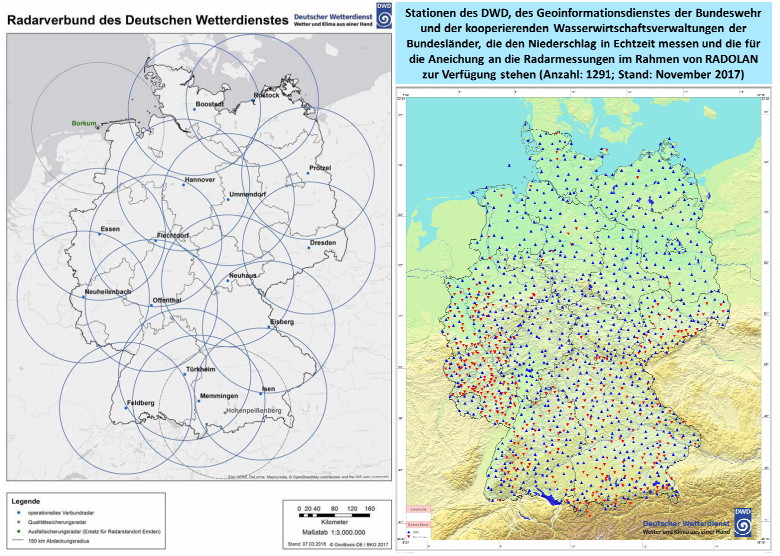
\includegraphics[width=0.6\textwidth,angle=0]{abb/daten_stationsuebersicht}
 \caption[Stationen Übersicht]{Übersicht über alle Boden und Radarstationen}
\label{fig:daten_stationsuebersicht}
\end{figure}

\noindent
Die RADOLAN Daten für die Netze werden über den Opendata Server vom DWD zur Verfügung gestellt. 
Die Binärdaten werden je nach Jahr in Form eines 1100x900 oder 900x900 Pixel Gitter über Deutschland gelegt.  
Dabei entspricht jeder Pixel 1km x 1km. Jeder Pixel in dem Pixel Koordinatensystem hat dabei zugehörige Höhen und 
Breitengrad Koordinaten. In Abbildung \ref{fig:radolan_koordinatensystem_aufbau} ist der Aufbau der Binärdaten zu sehen.
\begin{figure}[H]
 \centering
 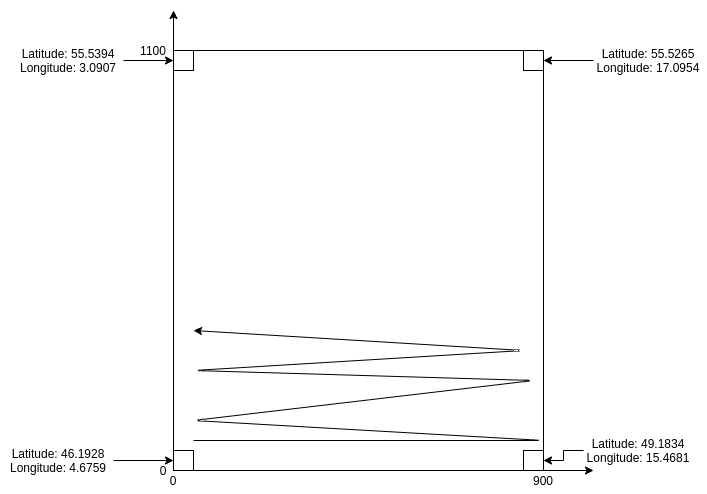
\includegraphics[width=0.8\textwidth,angle=0]{abb/radolan_koordinatensystem_aufbau}
 \caption[Aufbau des Koordinatensystems von Binärdaten]{Der Aufbau des Koordinatensystems der Radar Daten}
\label{fig:radolan_koordinatensystem_aufbau}
\end{figure}
Wie zu sehen ist, befinden sich der Pixel (0|0) in der Ecke unten links. Bei der Datenvorverarbeitung wird das Array mit 
den Pixeln jedoch von oben Links beginnend gefüllt, was bei dem entstehenden PNG  zu einer Spiegelung von 180 grad 
um die vertikale Achse führt (Siehe Kapitel Datenaufbereitung). 
Des Weiteren ist zu beachten, dass die Breitengrade in den Ecken nicht übereinstimmen.
So hat die Ecke unten Links einen größeren Breitengrad als die Ecke oben Links. 
Das Gleiche ist auch bei den Höhengraden zu beobachten. Die Ursache hierfür ist die Transformation der Daten von einer 
3D Kugel auf eine 2D Karte. In Abbildung \ref{fig:karte_abdeckung_daten} ist das daraus resultierende Ergebnis abgebildet. 

\begin{figure}[H]
 \centering
 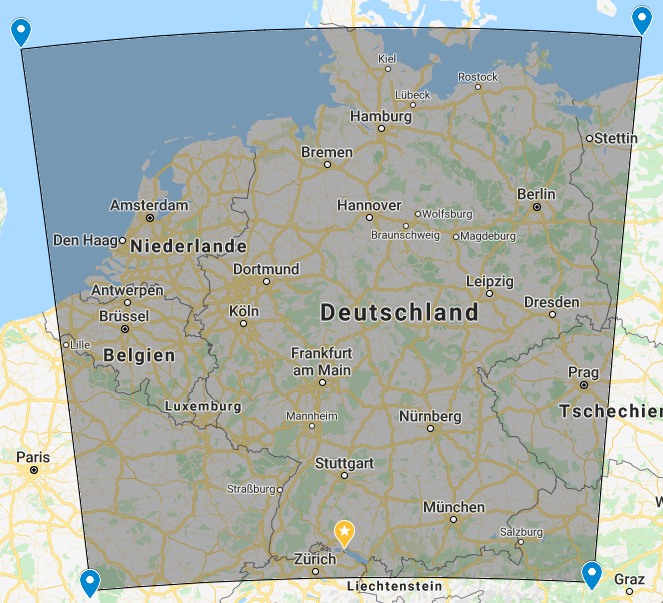
\includegraphics[width=0.6\textwidth,angle=0]{abb/karte_abdeckung_daten}
 \caption[Von Daten abgedeckte Fläche]{Die von den Daten abgedeckte Fläche auf einer 2D Karte}
\label{fig:karte_abdeckung_daten}
\end{figure}

\subsection{Die Qualität der Daten}
Um die Qualität der aus den RADAR Daten gewonnenen PNGs zu überprüfen, wurden die PNGs mit den Niederschlagsdaten von der 
Bodenstation in Konstanz verglichen. 
Die Daten der Station stehen in ein und zehnminütiger Auflösung zur Verfügung. 
Da bei der einminütigen Auflösung Daten Fehlen, wurden die Daten der zehnminütigen Auflösung verwendet.
Dafür musste aus den RADAR Daten jeder zweite Datensatz entfernt werden. 
Im ersten Schritt sollte die bereits berechnete Position von Konstanz, in dem Vorhersage PNG, bestätigt werden.
Dazu wurde die Korrelation zwischen der Regenstation in Konstanz und allen Pixel berechnet. 
Diese Korrelationen sind in Abbildung \ref{fig:karte_korrelation} grafisch dargestellt.
Dabei stellen hellere Farben eine höhere Korrelation dar. 
\begin{figure}[H]
    \centering
    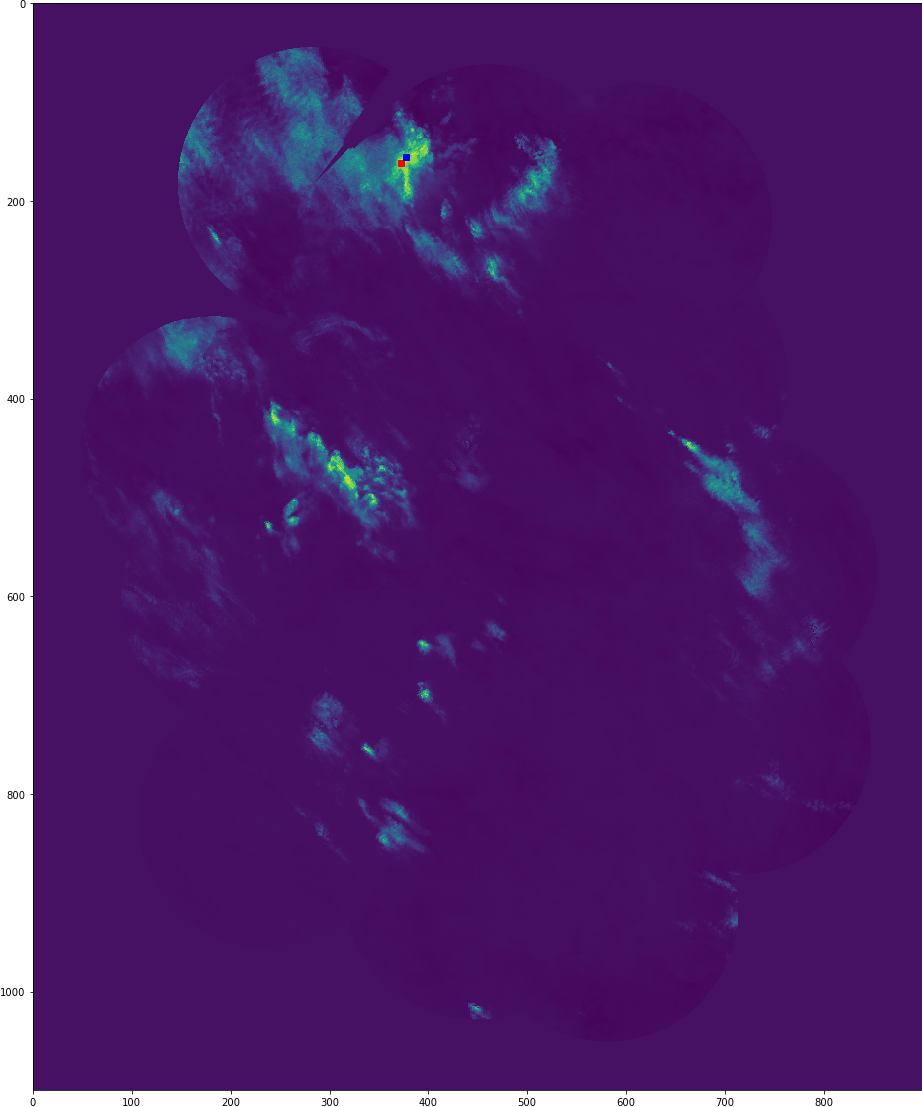
\includegraphics[width=0.8\textwidth,angle=0]{abb/Korrelation_Karte}
    \caption[Korrelationen der Regendaten in Kartenform]{Korrelation der Regendaten in Konstanz mit jedem Pixel}
   \label{fig:karte_korrelation}
\end{figure}

\noindent 
Das rote Quadrat stellt den Pixel mit der größten Korrelation dar, das blaue Quadrat den bisher berechneten Pixel von Konstanz. 
Die Abweichung dieser beiden Pixel voneinander lässt sich durch die kleine, für die Korrelation verwendete Datenmenge erklären. 
Wie man an der Position von Konstanz sieht, ist das Vorhersage PNG um 180 Grad an der vertikalen Achse gespiegelt.


\noindent
Um sicherzugehen, dass die für die Vorhersage verwendeten Daten mit dem tatsächlichen Niederschlag in Konstanz übereinstimmen, wurden sie grafisch dargestellt. 
In Abbildung \ref{fig:radar_station_daten_vergleich} ist der Niederschlag aus den RADAR Daten und der Bodenstation zu sehen. 
Es ist zu erkennen, dass die Regenstärke tendenziell leicht abweicht, während der Zeitpunkt des Regens sehr gut übereinstimmt.  
Die Abweichung der Intensität ist systematisch und sollte somit kein Problem darstellen. 
\begin{figure}[H]
    \centering
    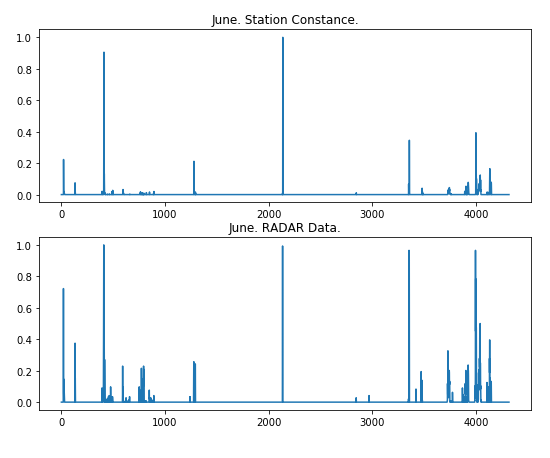
\includegraphics[width=0.6\textwidth,angle=0]{abb/radar_station_daten_vergleich_June}
    \caption[Radar und Stationsdaten]{Die Radar und Stationsdaten für Juni im Vergleich}
   \label{fig:radar_station_daten_vergleich}
\end{figure}

\noindent
In folgender Abbildung ist zu erkennen, dass die Regenstation in Konstanz im Juni 214 Zeitschritte mit Regen aufgezeichnet hat, es laut Radardaten aber 258 Zeitschritte mit Regen gab.
In 68\% der Regenzeitpunkte stimmen die Radar und Stationsdaten überein. 
Der fehlende Regen in den Stationsdaten könnte sich durch Messungenauigkeiten oder eine etwas abweichende geografische Lage von Konstanz erklären lassen.
\begin{figure}[H]
    \centering
    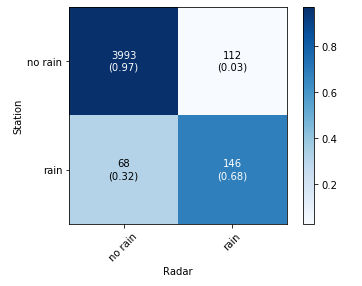
\includegraphics[width=0.6\textwidth,angle=0]{abb/confusion_matrix_stationdata_radardata}
    \caption[Confusion Matrix mit Radar und Stationsdaten]{Confusionmatrix für die Radar und Stationsdaten im Juni}
   \label{fig:confusion_radar_station}
\end{figure}
 